% By default, the contents of the back side of the final sheet is
% printed upside down. The option notumble suppresses that. Doing so
% may be necessary to suit the behavior of certain printing engines.
% Specifying [notumble] may also be useful during the writing of a
% document, to enable proof-reading on the screen.
\documentclass[notumble]{leaflet}
%\documentclass{leaflet}


\usepackage[english]{babel}
\usepackage[utf8]{inputenc}
\usepackage{lmodern}
\usepackage[T1]{fontenc}
\usepackage{amssymb}

\usepackage[default,scale=.82]{opensans}
% \renewcommand{\seriesdefault}{cl}
\renewcommand{\bfdefault}{sb}
% \renewcommand{\ttdefault}{fos}
\renewcommand\ttfamily{%
  \fontfamily{\ttdefault}%
  % \fontseries{lc}%
  \fontshape{\shapedefault}%
  \selectfont}

\usepackage{enumitem}
\setlist{
    topsep=0pt,
    partopsep=0pt,
    parsep=1ex,
    nolistsep,
    itemsep=.1ex
}
\setlength{\parskip}{1ex}

% \newcommand{\myparagraph}[1]{\vspace{.6em}\textsc{#1}}
\newcommand{\myparagraph}[1]{#1---}

\usepackage[table,svgnames]{xcolor}
\usepackage{graphicx}
\usepackage{tabularx,booktabs}
\usepackage{alltt,textcomp}
\usepackage{url}
\urlstyle{sf}
\usepackage{ifthen}
\usepackage{xspace}

\newcommand{\eg}{\emph{e.g.,}\xspace}
\newcommand{\ie}{\emph{i.e.,}\xspace}
\newcommand{\etal}{\emph{et al.,}\xspace}
\newcommand{\ct}[1]{{\textsf{#1}}\xspace}

\usepackage{microtype}

\definecolor{light-gray}{rgb}{0.8,0.8,0.8}
\definecolor{comment}{rgb}{0.35,0.35,0.35}
\definecolor{string}{rgb}{0.5,0,0.5}
\definecolor{darkRed}{rgb}{0.5,0,0}
\definecolor{darkBlue}{rgb}{0,0,0.3}
\definecolor{darkCyan}{rgb}{0,0.3,0.3}

\makeatletter
\newsavebox{\code@box}
 \newenvironment{displaycode}{%
     \par
     % \begin{lrbox}{\code@box}%
     \hspace{1.5em}\begin{minipage}{\linewidth}
       \begin{alltt}\small}{
       \end{alltt}
     \end{minipage}
     % \end{lrbox}
     % \usebox{\code@box}%
     \par}
\makeatother


% Use of english prevents babel from adding spaces before $:
\newcommand{\code}[1]{\foreignlanguage{english}{\texttt{#1}}}

\graphicspath{{./figures/}}

\title{\vspace{-1.0cm}\normalfont

\includegraphics[width=0.8\linewidth]{logo.pdf}
\\[1.2\baselineskip]%
\vspace{-0.8cm}
\fontseries{cl}\selectfont\LARGE
An innovative, open-source Smalltalk-inspired \\ language for live programming\\
\url{http://www.pharo.org}}
\date{}
\setmargins{7.8mm}{7.8mm}{7.8mm}{7.8mm}
\CutLine*{1} \CutLine*{2} \CutLine*{3} \CutLine*{4} \CutLine*{5}\CutLine*{6}

\begin{document}
\maketitle
\thispagestyle{empty}
\vspace{-1.7cm}
Pharo is both an \emph{object-oriented}, \emph{dynamically-typed}
general-purpose language and its own programming environment. The
language has a simple and expressive syntax which can be learned
in a few minutes. Concepts in Pharo are \emph{very consistent}:
\begin{itemize}
  \item Everything is an object: buttons, colors, arrays, numbers, classes, methods\ldots \emph{Everything!}
  \item A small number of rules, no exceptions!
\end{itemize}

\paragraph{Main Web Sites}
\begin{description}
 \item[Code hosting] \url{http://smalltalkhub.com}
 \item[Questions]    \url{http://discord.gg/Sj2rhxn}
 \item[Blog] \url{http://pharoweekly.wordpress.com}
 \item[Contributors] \url{http://pharo.org/about}
 \item[Topics]       \url{http://topics.pharo.org}
 \item[Consortium]   \url{http://consortium.pharo.org}
 \item[Association]  \url{http://association.pharo.org}
\end{description}

\subsection{PharoBooks}

\textbf{Pharo books} are available at: \url{http://books.pharo.org}\\
Pharo By Example, Deep into Pharo, Enterprise Pharo: a Web Perspective,
Numerical Methods in Pharo, TinyBlog Tutorial, Dynamic Web Development in Seaside 
(\url{http://book.seaside.st})

\textbf{More books} \url{http://stephane.ducasse.free.fr/FreeBooks}



%\pagebreak{}


\subsection{Minimal Syntax}
\noindent
\begin{tabularx}{\linewidth}{@{}rX@{}}
        \toprule
        \multicolumn{2}{c}{Six reserved words only}\\
        \midrule
        \textcolor{darkRed}{\code{nil}} & the undefined object\\
        \textcolor{darkRed}{\code{true}}, \textcolor{darkRed}{\code{false}} & boolean objects\\
        \textcolor{darkCyan}{\code{self}} & the receiver of the current message\\
        \textcolor{darkCyan}{\code{super}} & the receiver, in the superclass context\\
        \textcolor{darkCyan}{\code{thisContext}} & the current invocation on the call stack\\
\end{tabularx}

\subsection{Minimal Syntax (II)}
\noindent
\begin{tabularx}{\linewidth}{@{}rX@{}}
        \toprule
        \multicolumn{2}{c}{Reserved syntactic constructs}\\
        \midrule
        \textcolor{comment}{\code{"}{comment}\code{"}} & \\
        \textcolor{string}{\code{'}{string}\code{'}} & \\
        \textcolor{string}{\code{\#symbol}} & unique string \\
        \textcolor{darkRed}{\code{\$a}}, Character space & the character \textcolor{darkRed}{\code{a}} and a space \\
        \textcolor{darkRed}{\code{12 2r1100 16rC}} & twelve (decimal, binary, hexadecimal)\\
        \textcolor{darkRed}{\code{3.14 1.2e3}} & floating-point numbers\\
        \code{\#(\textcolor{string}{abc} \textcolor{darkRed}{123})} & literal array with the symbol \textcolor{string}{\code{\#abc}} and the number \textcolor{darkRed}{\code{123}} \\
        \code{\{\textcolor{darkBlue}{foo}\,.\ \textcolor{darkRed}{3}\,+\,\textcolor{darkRed}{2}\}} & dynamic array built from 2 expressions\\
        \code{\#[\textcolor{darkRed}{123 21 255}]} & byte array \\
        \code{\emph{exp1}. \emph{exp2}} & expression separator (period)\\
        \code{;} & message cascade (semicolon)\\
        \code{var := \emph{expr}} & {assignment} \\
        \code{\textasciicircum\ \emph{expr}} & return a result from a method (caret)\\
        \code{[\,:\textcolor{darkBlue}{p}\,|\,}\emph{expr}\code{\,]} & code block with a parameter \\
        \code{|\,\textcolor{darkBlue}{foo bar}\,|} & declaration of two temporary variables \\
        \bottomrule
\end{tabularx}

%\clearpage

\subsection{Message Sending}
When we send a message to an object, the message
\emph{receiver}, the method is selected and executed; the message returns an object. Messages syntax mimics
natural languages, with a subject, a verb, and complements. 


\noindent
\begin{tabularx}{\linewidth}{@{}lX@{}}
        \toprule
        \textbf{Java} & \textbf{Pharo}\\
        %\multicolumn{2}{c}{\textbf{Conditionals}}\\
        \midrule
      aColor.setRGB(0.2,0.3,0) & aColor r: 0.2 g: 0.3 b: 0 \\
      d.put("1", "Chocolate");& d at: '1' put: 'Chocolate'.\\
       \midrule
\end{tabularx}


\subsection{Three Types of Messages: Unary, Binary, and Keyword}

A \textbf{unary message} is one with no arguments.

\noindent
\begin{tabularx}{\linewidth}{@{}lX@{}}
        \toprule
      \textcolor{darkBlue}{Array} new.& $\rightsquigarrow$ anArray \\
      \#(\textcolor{darkRed}{4 2 1}) size.& $\rightsquigarrow$ 3\\
       \midrule
\end{tabularx}

\code{new} is an unary message sent to classes (classes are objects). 

A \textbf{binary message} takes only one
argument and is named by one or more symbol characters from \code{+}, \code{-}, \code{*}, \code{=}, \code{<}, \code{>}, ...

\noindent
\begin{tabularx}{\linewidth}{@{}lX@{}}
        \toprule
      \textcolor{darkRed}{3} + \textcolor{darkRed}{4}& $\rightsquigarrow$ 7 \\
     \textcolor{string}{'Hello'} , \textcolor{string}{' World'}& $\rightsquigarrow$ 'Hello World'\\
       \midrule
\end{tabularx}


The \code{+} message is sent to the object
\textcolor{darkRed}{\code{3}} with \textcolor{darkRed}{\code{4}} as
 argument. The string \textcolor{string}{\code{'Hello'}} receives the message \code{,}
(comma) with \textcolor{string}{\code{'~World'}} as the argument.

A \textbf{keyword message} can take one or more
arguments that are inserted in the message name.

\noindent
\begin{tabularx}{\linewidth}{@{}lX@{}}
        \toprule
     \textcolor{string}{'Pharo'} allButFirst: \textcolor{darkRed}{2}.& $\rightsquigarrow$ 'aro' \\
     \textcolor{darkRed}{3} to: \textcolor{darkRed}{10} by: \textcolor{darkRed}{2}.& $\rightsquigarrow$ (3 to: 10 by: 2)\\
       \midrule
\end{tabularx}

The second example sends
\code{to:by:} to \textcolor{darkRed}{\code{3}}, with arguments
\textcolor{darkRed}{\code{10}} and \textcolor{darkRed}{\code{2}}; this
returns an interval containing \textcolor{darkRed}{\code{3}},
\textcolor{darkRed}{\code{5}}, \textcolor{darkRed}{\code{7}}, and
\textcolor{darkRed}{\code{9}}.

\subsection{Message Precedence}

Parentheses\,$>$\,unary\,$>$\,binary\,$>$\,keyword, and finally from
left to right.

\noindent
\begin{tabularx}{\linewidth}{@{}lX@{}}
        \toprule
    (\textcolor{darkRed}{15} between: \textcolor{darkRed}{1} and: \textcolor{darkRed}{2}\,+\,\textcolor{darkRed}{4}\,*\,\textcolor{darkRed}{3}) not& $\rightsquigarrow$ false \\
       \midrule
\end{tabularx}



Messages \code{+} and \code{*} are sent first, then \code{between:and:} is sent, and \code{not}.
The rule suffers no exception: operators are just binary messages with \emph{no notion of mathematical precedence}.
\code{\textcolor{darkRed}{2}\,+\,\textcolor{darkRed}{4}\,*\,\textcolor{darkRed}{3}} reads left-to-right and gives \textcolor{darkRed}{18}, not \textcolor{darkRed}{14}!

%\clearpage

\subsection{Cascade: Sending Muliple Messages to the Same Object}

Multiple messages can be sent to the same receiver with \code{;}.

\begin{displaycode}
\textcolor{darkBlue}{OrderedCollection} new
  add: \textcolor{string}{#abc};
  add: \textcolor{string}{#def};
  add: \textcolor{string}{#ghi}.
\end{displaycode}

The message \code{new} is sent to \code{\textcolor{darkBlue}{OrderedCollection}} which
returns a new collection to which three
\code{add:} messages are sent. The value of the whole message cascade
is the value of the last message sent (here, the symbol
\textcolor{string}{\code{\#ghi}}). To return the receiver of the
message cascade instead (\ie the collection), make sure to send
\code{yourself} as the last message of the cascade.

\subsection{Blocks}
Blocks are objects containing code that is executed on demand. They are the basis for control structures like
conditionals \& loops.

\begin{displaycode}
\textcolor{darkRed}{2} = \textcolor{darkRed}{2}
  ifTrue: [ \textcolor{darkBlue}{Error} signal: \textcolor{string}{'Help'} ].
\end{displaycode}
\begin{displaycode}
\#(\textcolor{string}{'Hello World'} \textcolor{darkRed}{\$!})
  do: [ :\textcolor{darkBlue}{e} | \textcolor{darkBlue}{Transcript} show: \textcolor{darkBlue}{e} ]
\end{displaycode}

The first example sends the message \code{ifTrue:} to the boolean
\textcolor{darkRed}{\code{true}} (computed from
\code{\textcolor{darkRed}{2} = \textcolor{darkRed}{2}}) with a block
as argument. Because the boolean is \textcolor{darkRed}{\code{true}},
the block is executed and an exception is signaled. The next example
sends the message \code{do:} to an array. This evaluates the block
once for each element, passing it via the \code{e} parameter. As a
result, \code{\textcolor{string}{Hello~World!}} is printed.


\section{Common Constructs}

\noindent
\begin{tabularx}{\linewidth}{@{}lX@{}}
        \toprule
        \multicolumn{2}{c}{\textbf{Conditionals}}\\
        \midrule
        if (condition) & condition \\
      \ \ \   \{ action(); \} &   \ \ \ \ \    ifTrue: [ action ] \\
      \ \ \     else \{ anotherAction(); \}&\ \ \ \ \  ifFalse: [ anotherAction ]\\
       \midrule
      while (condition) \{ action(); &\ \  [ condition ] whileTrue:\\
      \ \ \     anotherAction(); \}&\ \ \ \ \ \ \  [ action. anotherAction ]
\end{tabularx}

\noindent
\begin{tabularx}{\linewidth}{@{}lX@{}}
        \toprule
        \multicolumn{2}{c}{\textbf{Loops/Iterators}}\\
        \midrule
         for(int i=1; i<11; i++)\{ & 1 to: 11 do: [ :i | \\
      \ \ \ \    System.out.println(i); \}&\ \ \ \ Transcript show: i ; cr ] \\
      \midrule
String [] names =\{"A", "B", "C"\};& | names | \\  
for( String name : names ) \{ &names := \#('A' 'B' 'C').\\
   \ \      System.out.print( name ); & names do: [ :each |\\
    \ \     System.out.print(","); \} & \ \ \ Transcript show: each, ' , ' ]\\
     \midrule
\end{tabularx}

Collections start at 1. Messages \code{at: index} gives element at index and \ct{at: index put: value} sets element at index to value.

\noindent
\begin{tabularx}{\linewidth}{@{}lX@{}}
     \toprule
      \multicolumn{2}{c}{\textbf{Collections}}\\
      \midrule
     \textcolor{string}{\#(4 2 1) at: 3}& $\rightsquigarrow$ 1 \\
     \textcolor{string}{\#(4 2 1) at: 3 put: 6}& $\rightsquigarrow$ \#(4 2 6) \\
     \textcolor{string}{Set new add: 4; add: 4; yourself}& $\rightsquigarrow$ aSet \\
     \midrule
\end{tabularx}

\noindent
\begin{tabularx}{\linewidth}{@{}lX@{}}
     \toprule
     \multicolumn{2}{c}{\textbf{Files and Streams}}\\
      \midrule
work := FileSystem disk workingDirectory. \\
stream := (work / 'foo.txt') writeStream. \\
stream nextPutAll: 'Hello World'. \\
stream close. \\
stream := (work / 'foo.txt') readStream. \\
stream contents. & $\rightsquigarrow$ 'Hello World' \\
stream close.
\end{tabularx}

%\clearpage
\section{Pharo: a Live Programming Environment}

Pharo comes with an integrated development environment. Pharo
is a \emph{live programming environment}: you can modify your objects
and your code while your program is executing. All Pharo tools are
implemented in Pharo:
\begin{itemize}
\item a code browser with refactorings;
\item a debugger, a workspace, and object inspectors;
\item and much, much more!
\end{itemize}

Code can be inspected and evaluated directly in the image, using
simple key combinations and menus (open the contextual menu on any
selected text to see available options).

% \begin{center}
%   \includegraphics[width={.6}\textwidth]{workspace}
% \end{center}

\subsection{The 5 Panes Pharo Code Browser}

\begin{center}
  \includegraphics[width=0.9\textwidth]{nautilus-anotated}
\end{center}

\begin{itemize}
\item The \emph{packages} pane shows all the packages of the system.
\item The \emph{classes} pane shows the class hierarchy of the
  selected package; the \emph{class side} checkbox allows for getting
  the methods of the metaclass.
\item The \emph{protocols} pane groups the methods of the selected
  class to ease navigation.  When a protocol name starts with a \emph{*}, methods of this
  protocol belong to a different package (\eg the \emph{*Fuel}
  protocol groups methods that belong to the \emph{Fuel} package);
\item The \emph{methods} pane lists the methods of the selected
  protocol; icons are clickable and trigger special actions;
\item The \emph{source code} pane shows the source code of the
  selected method. 
\end{itemize}


\subsection{Defining a class}
To add a class, edit the proposed template!
The following expression defines the class \code{Counter} as a subclass of \code{Object}.
It defines two instance variables \code{count} and \code{initialValue} inside the package \code{MyCounter}.

\begin{displaycode}
Object subclass: #Counter
   instanceVariableNames: 'count initialValue'
   classVariableNames: '' 
   package: 'MyCounter'
\end{displaycode}

The method \code{initialize} is automatically invoked when a new instance is created by sending the message \code{new} to the class i.e., \code{Counter new}.   

\begin{displaycode}
\textit{Counter >>} initialize 
    super initialize.
    count := 0. 
\end{displaycode}

\code{\textcolor{darkBlue}{\textit{Counter}\,>{}>\,}initialize} is a \textit{notation} to indicate that the following text is the content of the method \code{\textbf{initialize}} in the class \code{\textcolor{darkBlue}{Counter}}.

\subsection{Methods}
Methods are public and virtual. There are always looked up in the class of the receiver. By default a method returns \code{self}. 
Class methods follow the same dynamic lookup than instance methods. 
Method \code{factorial} defined in class \ct{Integer}. 

\begin{displaycode}
\textit{Integer >>} factorial
   "Answer the factorial of the receiver."
   self = 0 ifTrue: [^ 1].
   self > 0 ifTrue: [^ self * (self - 1) factorial].
\end{displaycode}

%\pagebreak{}

%\vspace*{\fill}


\subsection{Unit testing}
A test must be implemented in a method whose name starts with \code{test} and in a class that
inherits from \code{TestCase}.

\begin{displaycode}
\textcolor{darkBlue}{\textit{OrderedCollectionTest}\,>>}\,testAdd
  | \textcolor{darkBlue}{added} |
  \textcolor{darkBlue}{added} := \textcolor{darkBlue}{collection} add: \textcolor{string}{'foo'}.
  \textcolor{darkCyan}{self} assert: (\textcolor{darkBlue}{collection} includes: \textcolor{string}{'foo'}).
\end{displaycode}

The second line declares the variable \code{\textcolor{darkBlue}{added}}. The message \code{assert:} expects a true value.

\section{A simple, uniform and powerful model}

Pharo has a simple dynamically-typed object model:
\begin{itemize}
\item everything is an object --- instance of a class;
\item classes are objects too and there is single inheritance between classes;
\item traits are groups of methods that can be reused orthogonally to inheritance;
\item instance variables are protected; methods are public and virtual;
and blocks are lexical closures.
\end{itemize}

\textbf{Less is more:} There is no type declaration, no primitive
objects, no generic types, no modifiers, no operators, no inner
classes, no constructor, and no static methods. You will never need them in
Pharo!



%\vfill{}

\end{document}

%%% Local Variables:
%%% mode: latex
%%% TeX-master: t
%%% End:
